\chapter{Interviews with CLAI Members}\label{appendix:Bergenholtz}
The Center for Language Generation and AI (CLAI) at Aarhus University is dedicated to researching and developing foundational language models. CLAI explores the implications of these models for understanding language and cognition, and addresses the ethical issues inherent in language generation and AI. Additionally, the center investigates the creative and pedagogical potential of these technologies. CLAI is a cross-disciplinary research program that integrates linguistics, humanities computing, cognitive science, media studies, and aesthetics.

As preparation for this bachelor's thesis, interviews were conducted with members of CLAI to gain insights into the current research and application of LLMs within the university. Furtherly, inspiration was sought for the development of a chatbot, specifally the issues and challenges that arise when implementing such a system in an academic setting.
Interviews were conducted with the following members of CLAI:

\section*{Customized RAG Chatbot at Aarhus University}
    Associate professor Carsten Bergenholtz from the Department of Management implemented, in collaboration with associate professor Oana Vuculescu, a RAG chatbot for his Philosophy of Science course at Aarhus University. For inspiration and guidance on the development of a RAG chatbot an informal interview was conducted with professor Bergenholtz. His involvement provided crucial insights that shaped the direction of the implementation of the chatbot related to this thesis.

    \subsection*{Interview Summary}

    During our discussions, concerns were raised about the use of chatbots like ChatGPT-4 in educational environments. While these systems can produce impressive outputs, they also pose risks due to potential inaccuracies and a lack of course-specific knowledge. However, solutions exist to mitigate these challenges. Professor Bergenholtz shared his experience with implementing a customized RAG chatbot for his Philosophy of Science course, which had an enrollment of 550 students.

    \subsection*{Chatbot Implementation}

    The customized chatbot was used approximately 20,000 times by the students, indicating strong engagement and utility. Professor Bergenholtz uploaded about 250 pages of course-relevant documents, from text to subtitles from his online lectures, to create a knowledge base for the chatbot. This setup, based on AU's Microsoft Azure platform, ensured that the chatbot was:

    \begin{itemize}
        \item GDPR compliant, adhering to data protection regulations.
        \item Based on the ChatGPT-4 model, ensuring advanced conversational capabilities.
        \item Freely accessible to all students, removing financial barriers.
        \item Equipped with an appealing user interface, enhancing user experience.
        \item Integrated within the existing university systems, ensuring seamless access.
    \end{itemize}
    \begin{figure}[H]
        \centering
        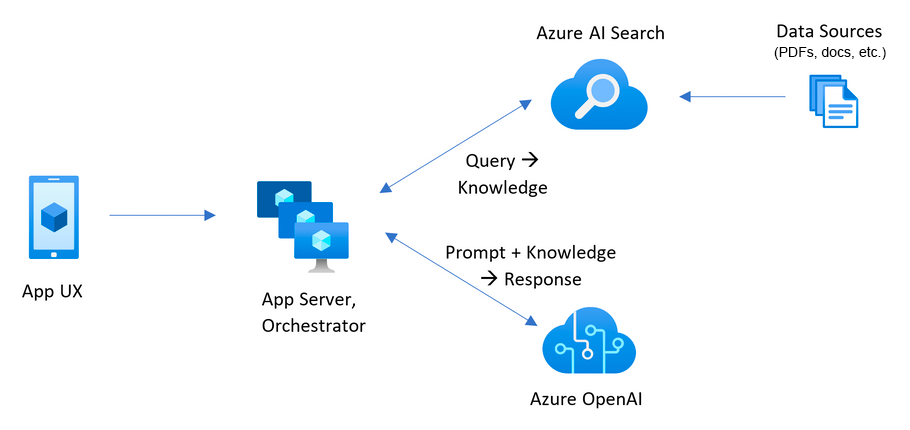
\includegraphics[width=0.6\textwidth]{figs/appcomponents.png}
        \caption{RAG patterns that include Azure AI Search from which Bergenholtz' chatbot was inspired from - taken from \cite{microsoft}}
        \label{fig:CLAI_Poster_Competition}
    \end{figure}

    The RAG chatbot was specifically designed to respond only to queries related to the course content. Questions outside the course scope received a 'cannot answer this' response to maintain the focus and academic integrity of the tool. Additionally, the chatbot provided a link to the source of its answers, enhancing transparency and trust.

    \subsection*{Chatbot Evaluation and Costs}

    The quality of the chatbot's responses was satisfactory, with about 85\% of interactions leading to useful answers, and only 2-4.5\% of responses being flawed. Notably, the flawed responses were quickly identified by users through follow-up questions. Despite its imperfections, the chatbot was considered a significant improvement over traditional search methods or regular chatbots used by students. The total cost of the chatbot was approximately 600€, with actual running costs around 400€ for 20,000 interactions, showcasing its cost-effectiveness.

    \subsection*{Student Feedback and Future Prospects}

    The chatbot was well-received based on survey responses, with students appreciating its ability to clarify complex concepts, compare texts, and summarize content. This tool proved particularly useful for large classes and when copyright for the necessary materials was held by the course instructor. Plans are in place to continue and enhance this service in future courses, focusing on guiding students to ask more effective questions.

    \subsection*{Conclusion}

    The implementation of the RAG chatbot at Aarhus University exemplifies the practical application of LLMs in enhancing educational experiences. The project set a precedent for future educational tools that leverage AI to support learning and inquiry. This initiative highlights the synergy between innovative technology and traditional educational practices, paving the way for more dynamic and interactive learning environments.

\section*{Introduction to Various Tools and Platforms for Development and Research of LLMs}
    Research assistant Rasmus Hansen from the Centre for Educational Development at Aarhus University specialises in research on students and teachers' practice with learning technology. His current focus is specifically on Generative AI, writing, and feedback. The interview with Rasmus provided valuable insights into some tools and platforms that can be used for developing and researching LLMs.
    \subsection*{Interview Summary}
        After presenting the goal of the thesis and the planned implementation of the chatbot, Rasmus provided an overview of the tools and platforms that could be beneficial for the project. The following tools/platforms were recommended:
        \begin{itemize}
            \item \textbf{Hugging Face:} A platform that provides access to pre-trained models, datasets, and training pipelines for NLP tasks.
            \item \textbf{GPT4ALL:} A free-to-use, locally running, privacy-aware chatbot where no GPU or internet is required. Furtherly, a guide on how use RAG in GPT4ALL was provided.\footnote{\url{https://docs.gpt4all.io/gpt4all_chat.html}}
            \item \textbf{LMStudio:} A platform that allows users to create, train, and deploy custom language models locally.
        \end{itemize}
        As the project progressed only the Hugging Face platform was used for this thesis. The platform provided access to the pre-trained BART model, and allowed for fine-tuning on custom datasets. The introduction to Hugging Face was instrumental in easy access to the BART model and the implementation of the case study: Low Rank Approximation.